\clearpage
\section{Dynamics and Control Module Details}

\subsection{Force Saturation}\label{sec:appendix-force-sat}
Section~\ref{sec:dynamics} introduced the use of describing functions to quantify the fundamental amplitude of non-sinusoidal force waveforms, which can achieve higher powers than the equivalent sinusoidal waveform for the same force limit.

The simulation permits the nonsinusoidal waveform to have a maximum fundamental a factor of $\frac{4}{\pi}$ above the force limit.
This coincides with the fundamental to peak ratio of a square wave, which is the limiting case both for the bang-singular-bang controller (a piecewise-discontinuous sine-square wave combination that \cite{hendrikx_optimal_2017} finds as the analytically optimal solution), and for the saturated sine controller (a piecewise-continuous sine-square wave combination that \cite{coe_initial_2020} finds as numerically optimal).
In fact, the optimization need not specify the exact nonlinear waveform, since under the describing function filtering hypothesis, only the fundamental matters for simulation purposes.
For hardware implementation purposes, the nonlinear controller can be obtained for the saturated-sine controller by the process outlined in \cite{mccabe_force-limited_2024}. 

MDOcean assumes that the saturated control impedance, and thus its fundamental, share the same phase as the optimal unsaturated controller (damping or reactive respectively).
This is optimal for the damping case, and slightly sub-optimal for the reactive case due to the presence of a small phase shift in the optimal saturated impedance and the matched impedance \cite{mccabe_force-limited_2024}.
The appropriate scale factor from the optimal unsaturated controller is found with numerical iteration. 

%Mathematically, a saturation factor $0< f_{sat}\leq 1$ is computed as the ratio between the fundamental amplitude of the saturated torque and the original unsaturated torque signal,
%\begin{equation}
%    f_{sat} = \min\left( \alpha\frac{\tau_{max}}{\tau}, 1\right),
%\end{equation}
%where $\tau_{max}$ is the maximum permissible generator torque and $\alpha$ is the ratio between the fundamental amplitude of the saturated waveform and the maximum torque $\tau_{max}$, using the describing function derived in \cite{mccabe_force-limited_2024},
%\begin{equation}
%    \alpha = \frac{2}{\pi} \left( \frac{F_p}{\tau_{max}}\sin^{-1}\frac{\tau_{max}}{F_p} +  \sqrt{1 - \left(\frac{\tau_{max}}{F_p}\right)^2} \right).
%\end{equation}
    
%When $\frac{F_p}{\tau_{max}}$ = 1 (no saturation), then $\alpha= 1$; when $\frac{F_p}{\tau_{max}} \rightarrow \infty$ (full saturation), then $\alpha= \frac{4}{\pi}$. This makes sense because $\frac{4}{\pi}$ is the harmonic amplitude of a unit square wave, and in full saturation the saturated signal approaches a square wave. $\alpha$ is plotted in Figure \ref{fig:alpha-fit}.

%The factor $f_{sat}$ describes the ratio of the saturated and unsaturated torque signal. Previous work \cite{mccabe_multidisciplinary_2022} implies that this is also the ratio of the saturated and unsaturated control gains, $m_{sat}$, but this is not the case because the WEC response also changes with saturation. 

% %Substituting $f_{sat}$ back into the equation of motion reveals that the control gain saturation multiplier $m_{sat}$ is the solution to a quadratic equation $a_q m_{sat}^2 + b_q m_{sat} + c_q = 0$. If the uncontrolled dynamics have a natural frequency $\omega_{n,u}$ and damping ratio $\zeta_u$, and the controlled unsaturated dynamics have natural frequency $\omega_n$ and damping ratio $\zeta$, then the quadratic coefficients can be expressed as:

% \begin{equation}\label{eq:abc-matrix}
%     \begin{bmatrix}
%         a_q \\ b_q \\ c_q
%     \end{bmatrix}
%     = 
%     \begingroup % keep the row spacing change local
%     \setlength\arraycolsep{2pt}
%     \begin{bmatrix} -4 & \frac{4}{f_{sat}^2} & \frac{1}{f_{sat}^2} & -1 & 0 & 0\\
%     8 & 0 & 0 & 2 & 8 & 2\\
%     -4 & -4 & -1 & -1 & -8 & -2 \end{bmatrix}
%     \endgroup
%     \begin{bmatrix} 
%  (\theta_1)^2  \\
%   (\theta_2)^2 \\
%    (\theta_3)^2 \\
%    (\theta_4)^2  \\
%    \theta_1 \theta_2 \\  
%     \theta_3 \theta_4
%     \end{bmatrix}
% \end{equation}
% where the basis vector $\vec{\theta}$ is a dimensionless function of the natural frequencies and damping ratios:
% \begin{equation}\label{eq:theta-basis}
%         \begin{bmatrix}
%   \theta_1  \\
%   \theta_2 \\
%    \theta_3 \\
%    \theta_4  \\
%     \end{bmatrix} =     \begin{bmatrix}
% ~ \overline{\omega} (\zeta_u - \overline{\omega}_n\zeta)  \\
%   \overline{\omega} ~\overline{\omega}_n \zeta \\
%   \overline{\omega}^2 - \overline{\omega}_n^2\\
%    \overline{\omega}_n^2 - 1  \\
%     \end{bmatrix}
% \end{equation}
% and the overlined frequencies indicate nondimensionalization by the uncontrolled natural frequency: $\overline{\omega} = \frac{\omega}{\omega_{n,u}}, \overline{\omega}_n = \frac{\omega_n}{\omega_{n,u}}$. The quadratic equation is then solved for $m_{sat}$, and of the two roots, the one that is real-valued and between 0 and 1 is used.

% The no saturation case ($f_{sat} = 1$) for \eqref{abc-matrix} yields $m_{sat}=1$. This confirms the expected behavior that when no force reduction is required, the powertrain coefficients can remain unchanged.

% Equations \eqref{eq:abc-matrix} and \eqref{eq:theta-basis} are an equivalent reformulation of \cite{mccabe_force-limited_2024}, which uses expressions for the complex reflection coefficient $\Gamma$ common in electrical engineering, rather than the damping ratio and natural frequency more common in mechanical engineering. The equivalence is:
% \begin{equation}
%     \Gamma = \frac{z-1}{z+1}, \quad z = \frac{2\theta_1 + i~ \theta_4}{-2(\theta_1+\theta_2) + i~(\theta_3+\theta_4)}
% \end{equation}
% % I am inputting zeta and omega_n corresponding to mechanical dynamcis when calculating m_sat, but I really should be inputting them corresponding to electrical dynamics. Maybe describe that?

% The gain saturation multiplier $m_{sat}$ is then used to modify the powertrain coefficients,
% \begin{align}
%     B_{p,sat} &= m_{sat} B_p, & K_{p,sat} &= m_{sat} K_p.
% \end{align}
% and these new control gains are then plugged into equation \eqref{eq:eom-freq-domain} to find the saturated displacement amplitude $X_{sat}$.

\begin{figure}
\centering
\includegraphics[width=.8\linewidth]{\matlabFilepath{35}}
\caption{Effect of Force and Power Limit}
\end{figure}

\clearpage
\subsection{Drag Model\label{sec:appendix-drag}}
Drag includes form drag (dominant impact), vortex shedding (moderate impact), and skin friction (minor impact) \cite{quartier_influence_2021}.
None of these three sources are captured in the MEEM hydrodynamics model due to the linear, irrotational, and inviscid assumptions respectively, so drag must be added separately.
As described in section \ref{sec:dynamics}, a describing function approximation is used.
This appendix describes an intricacy glossed over in section \ref{sec:dynamics} and entirely omitted in \cite{quartier_influence_2021}: the dependence of $\dot{x}_{wave}$ and thus $\dot{x}_{rel}$ across the width of the WEC in the direction of wave propagation $y$.
The authors of \cite{quartier_influence_2021} evaluate the wave velocity $\dot{x}_{wave}$ at the center of the WEC ($y=0$), which results in the drag damping coefficient $B_d$ becoming unrealistically low (even negative) at high frequencies and large wave heights.

A strip-theory approach avoids this issue by integrating the spatially-dependent infinitesimal drag force $dF_d$ over the wetted area $A_w$.
For a hollow cylinder of radius $R$ and inner radius $R_{in}$, this is expressed: 
% derived p156-159 notebook 3/10/25
% simplified p169-173 notebook 3/12/25
\begin{equation}\label{eq:drag-force-integral}
    F_d(t) = \int_{A_w} dF_d(y,t) = \int_{y=-R}^{R} w(y) P(y,t)dy
\end{equation}
where $w(y)$ is the local width of the WEC perpendicular to $y$:
\begin{equation}\label{eq:drag-width}
    w(y) = \begin{cases}
        2\sqrt{R^2-y^2}, & R_{in}<|y|<R \\
         2\sqrt{R^2-y^2}-2\sqrt{R_{in}^2-y^2}, &0<|y|< R_{in} \\
    \end{cases}
\end{equation}
and $P(y,t)$ is the local pressure acting vertically due to drag:
\begin{equation}\label{eq:drag-pressure}
    \begin{aligned}
    P(y,t) &= \frac{1}{2} \rho_w C_d ~\dot{x}_{rel}(y,t) ~|\dot{x}_{rel}(y,t)| \\
   &=  \frac{1}{2} \rho_w C_d ~\dot{X}_{rel}(y)^2 \sin(\omega t+\angle \dot{X}_{rel}(y)) ~\left| \sin(\omega t+\angle \dot{X}_{rel}(y))\right| \\
   &\approx  \frac{1}{2} \rho_w C_d ~\dot{X}_{rel}(y) ^2~\frac{8}{3\pi}\sin(\omega t+\angle \dot{X}_{rel}(y)) 
    \end{aligned}
\end{equation}
%notation: \dot{X}_rel here refers to the magnitude, not the complex phasor
% todo: I think technically the X's that I am taking the angle of should have a hat because they are complex

Moving into the frequency domain gives complex pressure $\hat{P}$:
\begin{equation}
\begin{aligned}
 \hat{P}(y,\omega)  &\approx \frac{1}{2} \rho_w C_d \frac{8}{3\pi}\alpha_v(y)^2 \dot{X}^2 e^{i\phi_\alpha(y)+i\angle\dot{X}}
    \end{aligned}
\end{equation}
where $\alpha_v(y)$ and $\phi_\alpha(y)$ are the amplitude and phase ratios, respectively, of the relative velocity and WEC velocity:
\begin{equation}\label{eq:drag-alpha-definitions}
\begin{aligned}
    \alpha_v(y) &\equiv \frac{\dot{X}_{rel}(y)}{\dot{X}} \\
    \phi_\alpha(y) &\equiv \angle
    \left(
        \frac{\hat{\dot{X}}_{rel}(y)}
            {\hat{\dot{X}}}
    \right)   
    = \angle\hat{\dot{X}}_{rel}(y) -  \angle\hat{\dot{X}} 
\end{aligned}
\end{equation}

Rewriting the relative velocity $\hat{\dot{X}}_{rel}(y)$ in equation \eqref{eq:drag-alpha-definitions} in terms of the finite depth incident wave velocity at a depth equal to the draft $\hat{\dot{X}}_{wave}(y) = \frac{H}{2} \frac{g k}{\omega} e^{-kT} e^{-iky}$ and the WEC velocity $\hat{\dot{X}}$ gives the following expressions for $\alpha_v^2(y)$ and $\phi_\alpha(y)$:

\begin{equation}
\begin{aligned}
    \alpha_v^2(y) &= 1 + r^2 e^{-2ky} - 2 r e^{-ky}  \sin\angle \hat{\dot{X}} \\
    \phi_\alpha(y) &= \mathrm{atan2}\left( \sin\angle \hat{\dot{X}} - r e^{-ky}, ~\cos\angle \hat{\dot{X}}\right) -  \angle\hat{\dot{X}}
\end{aligned}
\end{equation}
where $r = \dot{X}_{wave}(y=0)/ \dot{X}$ is the ratio of the wave velocity at the center of the WEC to the WEC velocity.
The drag force integral \eqref{eq:drag-force-integral} becomes:
\begin{equation}
    \hat{F}_d(\omega) \approx  \frac{1}{2} \rho_w C_d \frac{8}{3\pi}\dot{X}^2 e^{i\angle\hat{\dot{X}}}\int_{y=-R}^{R} w(y) \alpha_v(y)^2  e^{i\phi_\alpha(y)}dy
\end{equation}
noting that both the outer coefficient $e^{i\angle\hat{\dot{X}}}$ and the integral term $e^{i\phi_\alpha(y)}$ are complex phasors.
Setting $\hat{F}_{d}(\omega)%=\frac{1}{2}\rho_w C_d A_w \frac{8}{3\pi}  \dot{X}_{rel}(\omega)|\dot{X}_{rel}(\omega)|
=B_{d} \hat{\dot{X}} + K_{d} \hat{X}$ and solving for the coefficients yields
\begin{equation}\label{eq:drag-coeffs}
\begin{aligned}
B_{d} &= ~~~~~~\frac{4}{3\pi} \rho_w  C_{d} \dot{X} \int_{y=-R}^{R} w(y) \alpha_v(y)^2  \cos(\phi_\alpha(y))dy \\ % real part of c\_f
K_{d} &= - \omega~\frac{4}{3\pi} \rho_w  C_{d} \dot{X} \int_{y=-R}^{R} w(y) \alpha_v(y)^2  \sin(\phi_\alpha(y))dy \\ % -w times imag part of c\_f
\end{aligned}
\end{equation}

Plugging in the expressions for $w(y)$, $\alpha_v(y)$, and $\phi_\alpha(y)$ gives an integral with the following form:
\begin{equation}
\begin{aligned}
    &\int_{y=-R}^{R} w(y) \alpha_v(y)^2  e^{i\phi_\alpha(y)}dy \\
    = &\int_{y=-R}^{R} w(y) \sqrt{1 + r^2 e^{-2ky} - 2 r e^{-ky}  \sin\angle \hat{\dot{X}}} \left(f_3(\angle\hat{\dot{X}}) + f_2(\angle\hat{\dot{X}})re^{-ky}\right)  dy
\end{aligned}
\end{equation}
where $f_2$ and $f_3$ are trigonometric functions \hl{that I will derive during re-scrutineering, they are different for the cosine (Bd) vs sine (Kd).
For now before these integrals are derived, I assume the following:}
\begin{equation}
\begin{aligned}
    \phi_\alpha(y) &= 0 \\
    \alpha_v(y) &= \alpha_v(y=0) = 1 + r^2 - 2 r \sin\angle \hat{\dot{X}}
\end{aligned}
\end{equation}

Comparisons against WEC-Sim confirmed that this assumption yields more accurate results than the drag formulation used in \cite{quartier_influence_2021}, which uses an identical $\alpha_v(y)$ but assumes a different phase: $\phi_\alpha(y)=\phi_\alpha(y=0)$. 
At high frequencies and large wave heights, $r$ is large and $\phi_\alpha(y=0)$ exceeds $\pi$, causing the drag damping coefficient $B_d$ to be negative (non-dissipative), which is not realistic.
While setting $\phi_\alpha(y)=0$ does not guarantee that $B_d$ is always positive, it is found through testing to significantly reduce the risk of negative damping and to promote convergence of the drag loop.
In the optimization, any negative drag damping coefficents are set to zero.

% todo: write out full integral
%Like \cite{quartier_influence_2021}, this formulation evaluates the wave velocity $\dot{x}_{wave}$ at the center of the WEC rather than considering the variation in wave velocity along the direction of propagation as would be done with strip theory. This avoids cumbersome integral calculations at the cost of a small inaccuracy that will be quantified in section~\ref{sec:validation}.

With this approximation, the nonlinear time-domain drag equation is now a quasi-linear frequency-domain equation, since the state-dependence of the coefficients $B_{d}$ and $K_{d}$ prevents true linearity.
The solution for states $|\dot{X}|$ and $\angle \dot{X}$ can be obtained either through numerical iteration or analytical solution of the nonlinear equation\eqref{eq:eom}.
Iteration is chosen here, the same approach used for a frequency-domain drag simulation of floating offshore wind turbines \cite{hall_open-source_2022}.
Rather than employ a typical nonlinear root-finding algorithm, MDOcean simply uses the equation of motion \eqref{eq:eom} to obtain subsequent iterates.
This is a form of fixed point iteration where $x_k = g(x_{k-1})$ and is therefore guaranteed to converge as long as $|\frac{\partial g(x)}{\partial x}| < 1$ at the solution. %\hl{find a better place to cite for this besides wikipedia} \url{https://en.wikipedia.org/wiki/Root-finding_algorithm#Fixed_point_iteration_method}. 
Five to eight iterations on $|\dot{X}|$ and $\angle \dot{X}$ are typically required to converge all sea states to within 0.01~m, % from summer research slide 44 5/30/24
and a sample convergence plot is shown in Figure~\ref{fig:drag-convergence}.

In high-frequency sea states where there is substantial phase difference between $\dot{X}_{rel}$ and $\dot{X}$, $B_d$ occasionally becomes negative.
This does not violate the dissipative nature of drag \textit{overall}, because $F_d$ always opposes $\dot{X}_{rel}$ even if it does not oppose $\dot{X}$.
The non-dissipative effect of drag \textit{on the body} can be interpreted as modeling a second-order wave excitation force.
The effect would likely be mitigated if the position-dependence of the wave velocity were modeled, although this would require a difficult integration over the body surface and is left to future work.
Instead, if the negative drag exceeds the radiation damping and causes instability, the power for that sea state is zeroed.

Note that in the quasi-linear formulation, the lack of complete linearity means that the complex-conjugate reactive controller is technically no longer optimal.
The standard optimal control damping is derived by setting
\begin{equation}
0 = \frac{\partial P}{\partial B_p} = \frac{\partial \frac{1}{2} (B_p) \omega^2 |X|^2}{\partial B_p} = \frac{\partial \frac{1}{2} (B_p) \omega^2 |\frac{H\gamma/2}{(m+A_h)s^2+(B_h+B_d+B_p)s+(K_h+K_d+K_p)}|^2}{\partial B_p} 
\end{equation}
and the typical simplification $\frac{\partial B_d}{\partial B_p}=\frac{\partial K_d}{\partial B_p}=0$ must be replaced with the implicit dependence of $|X|$ on $B_d$ and $K_d$ from \eqref{eq:drag-coeffs}.
In practice, however, the standard complex conjugate controller was observed to produce nearly identical power as the one incorporating the more complicated dependence, so the standard is used for simplicity.

\begin{figure}
    \centering
    \includegraphics[width=0.75\linewidth]{\matlabFilepath{33}}
    \caption{Convergence plot for drag iteration}
    \label{fig:drag-convergence}
\end{figure}

\clearpage
\subsection{Slamming Amplitude}\label{sec:appendix-slam}
In regular waves of height $H$, the conditions for slamming can be derived by comparing the vertical position of the bottom of the WEC, $x(t)-\Delta z_{slam,bot}$, with the wave elevation $\zeta(y,t)$, which depends on the horizontal position coordinate $y$.
To prevent slamming, the criteria
\begin{equation}\label{eq:slamming-time-domain}
\begin{aligned}
    x(t) - \Delta z_{slam,bot} &< \zeta(y,t) \\ 
    |X|\cos(\omega t+\angle X) - \Delta z_{slam,bot} &< \frac{H}{2}\cos(\omega t - k y)
\end{aligned}
\end{equation}
must be true at all times and over all positions where the body could exit the waves, $-D/2<y<D/2$.
Note that this expression assumes a sinusoidal waveshape but still applies for irregular waves if a wave-by-wave approach \cite{lin_fast_2025} is utilized.
Manipulation yields the criterion $|X|<X_{slam}$, where the critical amplitude before slamming occurs $X_{slam}$ is
\begin{equation}
\begin{aligned}
    X_{slam} &= \sqrt{\Delta z_{slam,bot}^2-\left(\frac{H}{2}\sin\theta\right)^2 } - \frac{H}{2} \cos\theta \\
    \textrm{where } \theta &= \max\left(0,~ \frac{-kD}{2}+|\pi-\angle X|\right).
\end{aligned}
\end{equation}
This expression reduces to the simple limits $\Delta z_{slam,bot}-H/2$ and $\Delta z_{slam,bot}+H/2$ for short wavelengths $(\theta=0)$ and long wavelengths $(\theta=\pi)$ respectively.
These limits are also the minimum and maximum nonzero critical slamming amplitudes for any design and wave condition.
For intermediate wavelengths, the variable $\theta$ accurately accounts for the effect of body diameter and the phase offset of body motion from the waves.
Intuitively, $\theta$ represents how high up the free surface the bottom of the WEC is allowed to get before the edge exits the water, with $\theta=\pi$ allowing the body to get all the way to the wave crest (top) and $\theta=0$ requiring the float to remain fully below the trough (bottom).
Figure~\ref{fig:slam} visualizes the relationship using the nondimensional parameter $X^*$ to map the slamming amplitude onto the range $[-1,1]$.
This reveals that besides increasing the draft, increasing $\theta$ can prevent slamming, for example by decreasing the diameter or adjusting $\angle X$ via control.
If $\Delta z_{slam,bot}<H/2\sin\theta$, slamming occurs even for a stationary body, and the critical slamming amplitude is set to zero to indicate an unviable design.
\begin{figure}
    \centering
    \includegraphics[width=1\linewidth]{\matlabFilepath{34}}
    \caption{Nondimensional critical slamming amplitude}
    \label{fig:slam}
\end{figure}
%\hl{add description of similarities and differences of this to Budal's upper bound}

Separately, there exists a symmetrical counterpart to the above slamming condition, where in addition to requiring the bottom the WEC to remain below the waves, one can require that the top of the WEC remains above the waves, preventing full submersion. 
Analogous to \eqref{eq:slamming-time-domain}, we obtain:
\begin{equation}\label{eq:top-slamming}
    x(t) + \Delta z_{slam,top} > \zeta(y,t)
\end{equation}

Conceptually, both the bottom-slamming requirement \eqref{eq:slamming-time-domain} and the top-slamming requirement \eqref{eq:top-slamming} must be applied to both the float and the spar for a total of 4 constraints for each sea state.
However, the top-slamming and bottom-slamming requirement for each body is aggregated into a single constraint for each sea state, using $\Delta z_{slam}=\min(\Delta z_{slam,top}, \Delta z_{slam,bot})$, where the values for $\Delta z_{slam,top}$ and $\Delta z_{slam,bot}$ were given in \sectionautorefname~\ref{sec:dynamics}.
\hl{(Note: There also might be a slight difference in the way theta would be calculated for top and bottom slamming, this will be checked during re-scrutineering).}
%However, implementing the top-slamming requirement for the float becomes redundant of the float bottom-slamming requirement due to the parameter choice $T_{f,2}/h_f=1/2$ enforcing equal draft and above-water height.
%If $h_f$ were added as an independent design variable, the float top-slamming requirement would become necessary to implement, although note that the normalized value of $\frac{dLCOE^*}{dT_{f,2}/h_f}$ in \figureautorefname~\ref{fig:param-sens-J-star-tornado} is less than -0.1, suggesting that the addition of $h_f$ as a design variable would provide little benefit and is therefore low priority.
Meanwhile, it is only required to implement the slamming constraint for the float not the spar because \reqref{base_dynamic} and \reqref{tops_dynamic} already ensure, respectively, that the bottom of the spar remains below the bottom of the float and that the top of the spar remains above the top of the float across all dynamic conditions.
Since the float slamming requirement applies for all $-D_f/2<y<D_f/2$ and the spar diameter is always smaller than the float's (via \reqref{float_spar_diam}), the spar slamming requirements are redundant. This reduces the number of slamming constraints per sea state from four to one.

Following section~\ref{sec:discussion}, it is interesting to analyze the impact of the more complicated intermediate-wavelength slamming model compared to the simple and conservative short-wavelength model ($X_{slam}=\Delta z_{slam}-H/2; X^*=-1$).
Relevant model values for the minimum-LCOE float design are plotted for each sea state in \figureautorefname~\ref{fig:slamming-validation}.
Although the intermediate wavelengths ($X^*>-1$) occur for many operational sea states, those sea states are not the ones where the slamming constraint is active (where $X_{slam}/X-1 \approx 0$) because in this JPD, large amplitude waves occur only at high periods.
If the more conservative short-wavelength model is used, the slamming constraint appears violated with a value of $-0.08$ (the small blue portion at the top of the rightmost subplot at $T_e=12.5$ s, $H_s=6.75$ m), indicating that the float draft would need to increase by around 8\% to prevent slamming.
This would increase total material cost by around 2\% and LCOE by around 0.5\%, an effect likely dwarfed by other sources of uncertainty.
Thus, in this case the more complicated, less conservative slamming model has only a minor impact on the optimization, although more substantial impact is expected in seas with co-occurring large-amplitude and low-to-moderate-period waves. 
\begin{figure}
    \centering
    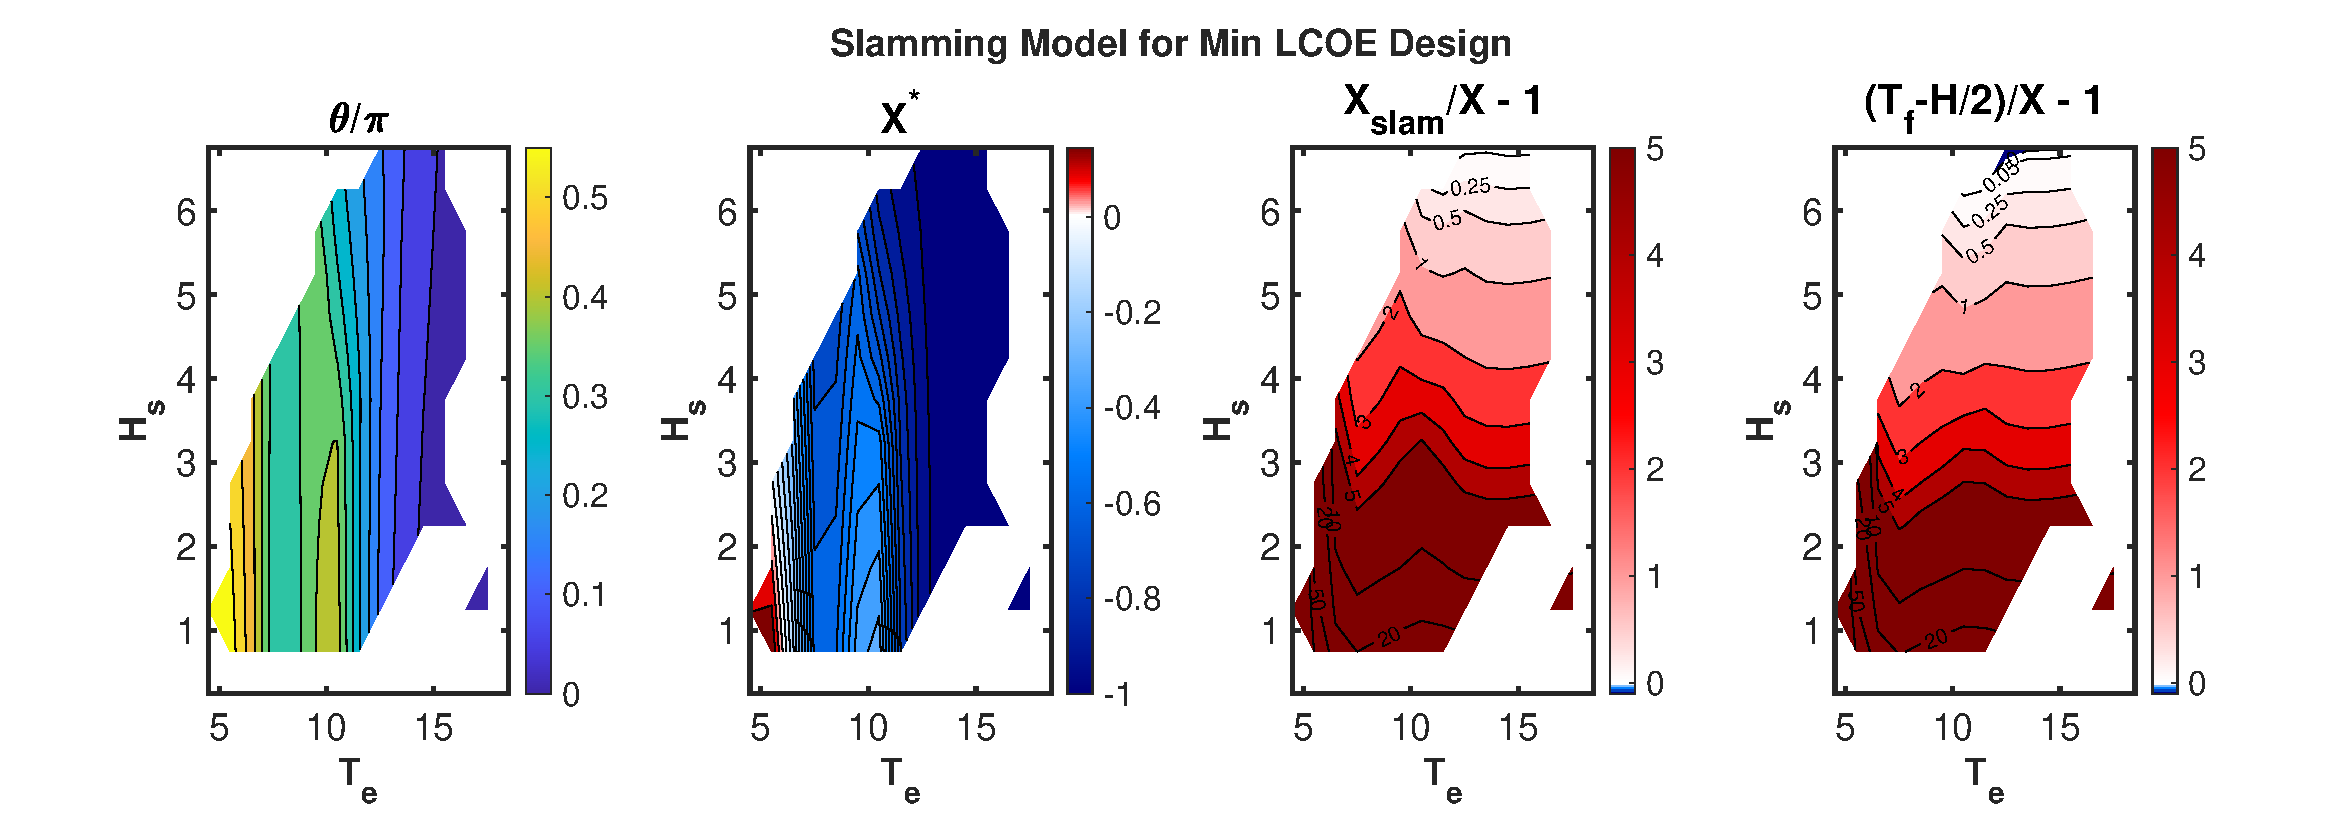
\includegraphics[width=1\linewidth]{figs/2025-04-11_10.21.55/slam_validation.pdf}
    \caption{Slamming Model Comparison for Minimum LCOE Design in Operational Sea States}
    \label{fig:slamming-validation}
\end{figure}



\clearpage
\subsection{Dynamic Validation using WEC-Sim}\label{sec:appendix-wecsim}
A WEC-Sim parallel multiple condition run is performed in accelerator mode for 3100s with a 100s ramp time using the ode4 solver and a 10 ms timestep, with the default mass properties of the WEC-Sim RM3 tutorial.
Each of the 210 sea states are simulated individually. %Table~\ref{tab:dynamic-validation} and 
Figure~\ref{fig:dynamic-validation} compares the results.
% \begin{table}
%     \centering
%     \begin{tabular}{|c|c|c|} \hline 
%          Power Percent Error: Average, Maximum&  $C_d=0$& $C_d=1$\\ \hline 
%          WAMIT&  1.90\%, 1.96\%& 5.21\%, -70\%\\ \hline 
%          MEEM&  -6.30\%, -14\%& -2.79\%, -80\%\\ \hline
%     \end{tabular}
%     \caption{Dynamic validation showing error in a variety of modeling assumptions}
%     \label{tab:dynamic-validation}
% \end{table}
\begin{landscape}
\begingroup
\begin{figure}
\centering
\begin{tabular}{c m{1em} | >{\centering\arraybackslash}m{.5\linewidth} >{\centering\arraybackslash}m{.5\linewidth} }
  && \multicolumn{2}{c}{Drag Coefficent}\\
         && $C_d=0$& $C_d=1$\\ \hline
    \multirow{2}{*}[-3em]{\rot{Hydro Coeffs}} &\rot{Identical}& \includegraphics[width=\linewidth]{\matlabFilepath{36_a}} & \includegraphics[width=\linewidth]{\matlabFilepath{36_b}} \\
     &\rot{Different} & \includegraphics[width=.5\linewidth]{example-image-a} & \includegraphics[width=\linewidth]{\matlabFilepath{36_d}} \\
\end{tabular}
\caption{Dynamic validation showing error in a variety of modeling assumptions}
\label{fig:dynamic-validation}
\fillandplacepagenumber
\end{figure}
\endgroup
\end{landscape}

\clearpage
\section{Structures Module Details}
\label{sec:appendix-structures}
Inputs to the structures module include forces, bulk and structural dimensions, and material constants.
It outputs a factor of safety for each limit case.
First, it obtains equivalent section properties based on the plate and stiffener dimensions.
Second, it relates applied loads to stresses and deflection using analytical solutions to structural boundary value problems obtained from the well-known Roark's handbook \cite{young_roarks_2001} and the references therein.
Finally, it utilizes design standards from organizations like Det Norske Veritas, the American Bureau of Shipping, and the American Iron and Steel Institute to develop limit state expressions for each possible failure mode of each major structural element under each design load case. %\hl{cite DNV standards, RM3 report+new structures addendum, some WEC structures paper, say that typically structures are designed to an ultimate limit and made of stiffened steel because it is efficient way to handle the spread out surface load of the ocean. Also note that for consistency with the RM3 report, welded joints are assumed everywhere, although using pinned joints such as a rod end attachment on the float and reaction plate tubular support structures could enhance structural efficiency.}

\subsection{Equivalent Section Properties for Stiffened Plates}\label{sec:equivalent-thickness}
Stiffeners are structural elements, frequently with I or T profiles, that can be welded or riveted to flat plates to provide additional load-carrying capacity and prevent buckling.
Stiffened plates are common in marine and aerospace structural design because they are an efficient way to carry spatially distributed fluid loads.
To analyze these compound sections, equivalent properties can be established that describe the overall bending stiffness of the combined section as if it were a simple uniform section, while still utilizing the maximum distance from the neutral axis of the irregular section to accurately determine stress.
Figure~\ref{fig:stiffened-plate} illustrates the concept of equivalent thickness for a stiffened plate.
\begin{figure}
    \centering
    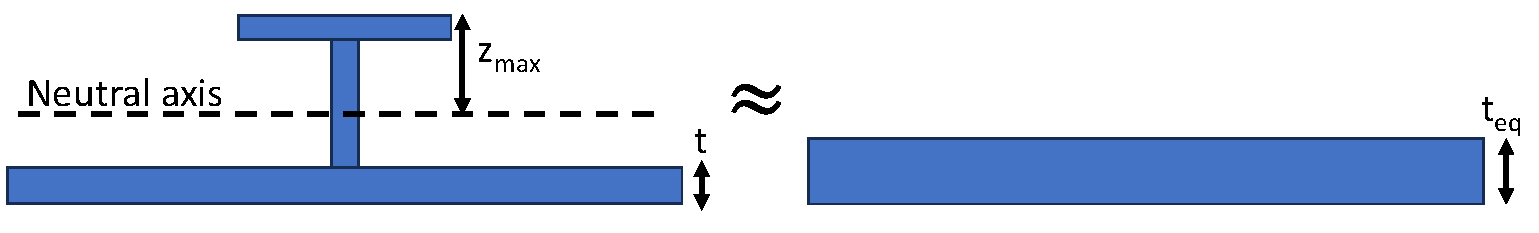
\includegraphics[width=\linewidth]{figs/stiffener_equivalence.pdf}
    \caption{Equivalent thickness for a stiffened plate}
    \label{fig:stiffened-plate}
\end{figure}

Specifically, the equivalent thickness of the plate $t_{eq}$ is derived by equating the stiffened section's second moment of area per unit width with that of a uniform section:
\begin{equation}
    \int z^2dz = \frac{t_{eq}^3}{12}
\end{equation}
Next, deflection of the stiffened plate is equal to the deflection of the equivalent unstiffened plate with flexural rigidity $D_{eq}$:
\begin{equation}
    D_{eq} = \frac{E~  t_{eq}^3}{12(1-\nu^2)}
\end{equation}

The maximum stress $\sigma$ of the stiffened plate is then:
\begin{equation}\label{eq:plate-stress}
    \sigma= 12M z_{max}/t_{eq}^3
\end{equation}
where $M$ is the maximum moment per unit length and $z_{max}$ is the maximum distance from the neutral axis of the stiffened section.
This parallels the stress for an unstiffened plate of thickness $t$, which is $\sigma=6M/t^2 = 12 M(t/2)/t^3$.

Note that this equivalent-thickness method of accounting for stiffeners assumes that as a whole, the stiffener-plate system deflects like a single plate element, rather than as set of multiple plate elements separated by stiffeners.
This is a reasonable assumption when the stiffeners are small and densely spaced with respect to the plate, but breaks down if the stiffeners come to dominate the system.
The so-called effective breadth ratio $\rho$ is used to quantify the validity of this assumption, where the equivalent-thickness method requires $\rho=1$:
\begin{equation}
   \rho = \rho_\lambda \rho_\psi
\quad 
\rho_\lambda = \begin{cases}
        1, & \lambda\leq 0.673 \\
        \frac{1-0.22/\lambda}{\lambda}, & \lambda > 0.673
    \end{cases} \quad
    \rho_\psi = \begin{cases}
        1, & \psi> -0.236 \\
        \frac{1}{2}+\frac{1}{3-\psi}, & \psi \leq -0.236
    \end{cases} 
\end{equation}
The effective breadth ratio depends on the slenderness factor $\lambda$ and load distribution factor $\psi$, found as follows:
\begin{equation}
\begin{aligned}
    \lambda &= \frac{1.052}{\sqrt{k_{buckle}}} \frac{w}{t} \sqrt{\frac{f_1}{E}} \\
    \psi&=\frac{f_2}{f_1}
    \end{aligned}
\end{equation}
with $t$ referring to the plate unstiffened thickness, $w$ as the distance between stiffeners, $f_1$ as the maximum compression stress along the width, and $f_2$ as the maximum tension stress along the width (or minimum compression stress, if there is no tension).
By convention, compression stress is positive and tension is negative, so $\psi$ ranges from $-\infty$ to $+1$.
The plate buckling coefficient $k_{buckle}$ is expressed as:
\begin{equation}\label{eq:k-buckle}
  k_{buckle} = 4+2\left(1-\psi\right)^3+2\left(1-\psi\right)
\end{equation}
This effective breadth procedure follows the American Iron and Steel Institute design manual \cite{american_iron_and_steel_institute_cold-formed_1991}.
Rather than enforcing $\lambda<0.673$, corresponding with $\rho_\lambda=1$, MDOcean more flexibly requires $\lambda<0.809$, corresponding to $\rho_\lambda=0.9$ and thereby capping the error due to insufficient slenderness at around 10\%.
MDOcean also uses $k_{buckle}=4$, the minimum value that equation \eqref{eq:k-buckle} can take on, conservatively maximizing the slenderness factor $\lambda$.

Broadening the design space to allow for more dominant stiffeners with higher slenderness factors would require modeling the stiffener-plate system not as a plate with the stiffeners absorbed into an equivalent thickness, but as individual stiffeners with the plate absorbed into the effective breadth.
That model has other complexities such as the shear lag phenomenon so is left to future extensions \cite{wierzbicki_lecture_2013,american_iron_and_steel_institute_cold-formed_1991}.

%\hl{Describe how this informs the lower design variable bounds on the structural stiffnesses.}

\subsection{Float}
The float is composed of 12 watertight stiffened shells in the shape of trapezoidal prisms.
Each shell consists of a top and a bottom trapezoidal plate, and an inner, an outer, and two side rectangular plates.
All edges are welded.
Rather than model the deflections of each edge and apply compatibility, for simplicity the edges of each plate are conservatively modeled as fixed.
The top and bottom plates are the only ones with external heave loads, arising from the float-spar tubular connection and the hydrodynamic pressure respectively.

The trapezoidal plates are isosceles trapezoids with smaller base $b_1 = \pi D_{f,in}/12$, larger base $b_2=\pi D_f/12$, and perpendicular height $h_0=(D_f-D_{f,in})/2$ (see \figurename~\ref{fig:trapezoid}).
The references consulted do not contain structural results for trapezoidal plates, so geometric intuition is used to scale available solutions.
For example, \cite{young_roarks_2001} contains models for rectangular plates under perpendicular loading.
They show that the maximum bending stress $\sigma$ scales with the square of the shorter side length, $x_{min}^2$. % in rectangular plates, with the square of the altitude in triangular plates, and with the square of the radius in circular sectors. 
This makes sense because for fixed-edge plates with distributed loads, it is the square of the minimum distance from an edge to the point of highest deflection, $(x_{min}/2)^2$, that geometrically sets the maximum curvature, so $\sigma\sim x_{min}^2$.
For trapezoids, one then expects approximate rectangles ($b_2/b_1\approx1$) to have $x_{min}=\min(b_1,h_0)$, short trapezoids ($h_0<b_1)$ to have $x_{min}=h_0$, tall trapezoids ($h_0\gg b_2$) to have $x_{min}=b_1$, and intermediate trapezoids to have an $x_{min}$ that depends on the trapezoid slope.
The nominal RM3 design falls into this intermediate case, with $b_1\approx1.7$~m, $b_2\approx5.2$~m, and $h_0\approx6.8$~m.
These dimensions are shown in figure~\ref{fig:trapezoid}.

\begin{figure}
    \centering
    \includegraphics[width=0.75\linewidth]{\matlabFilepath{37}}
    \caption{Trapezoidal float plate with inscribed circle used to determine $x_{min}$}
    \label{fig:trapezoid}
\end{figure}

To approximately capture the dimensions of a trapezoid which effectively set the deflection curvature and therefore stress, $x_{min}$ is set to the diameter of the largest circle that can be inscribed in the trapezoid tangent to the shorter base $b_1$.
This inscribed circle scheme satisfies all limit cases mentioned above and can be calculated as
\begin{equation}
    x_{min} = \begin{cases}b_1 \left( m + \sqrt{1+m^2}\right), & h_0 \geq \sqrt{b_1b_2} \\ h_0, & h_0 < \sqrt{b_1b_2}\end{cases}
\end{equation}
where $m=(b_2-b_1)/(2h_0)$ is the slope of the trapezoid.
The expression is continuous at $h_0=\sqrt{b_1b_2}$, the point where the inscribed circle becomes tangent to base $b_2$ in addition to $b_1$.
Continuity of the model across the design space avoids problems in the gradient-based optimization due to undefined gradients.
The inscribed circle model gives $x_{min}\approx2.2$~m for the nominal float design.
In addition to the shorter side length $x_{min}$, stress in a fixed-edge rectangular plate also depends weakly on the longer side length of the plate $x_{max}$, which for the trapezoid is taken as
\begin{equation}
    x_{max} = \begin{cases} h_0,& h_0 \geq \sqrt{b_1b_2} \\ \frac{b_1+b_2}{2} + h(1-\sqrt{1+m^2}), & h_0 < \sqrt{b_1 b_2}\end{cases}
\end{equation}
using a similar inscribed circle scheme to maintain continuity.
Under a distributed pressure $q$, the bottom plate maximum moment per unit length is then $M_{bot}=\beta q x_{min}^2$ for $\beta$ tabulated as a function of $x_{max}/x_{min}$ in reference \cite{timoshenko_theory_1959}, and the bending stress is found by plugging this moment into equation~\eqref{eq:plate-stress}.

The top float plate has equivalent thickness $t_{f,top,eq}$ and the same dimensions and edge fixity as the bottom plate.
Unlike the uniform pressure on the bottom plate, the top plate is subject to the welded tubular float-spar attachment force and moment, modeled as a load distributed over a small circle of radius $r_0$, where $r_0$ is assumed to be at least half the thickness.
Under these conditions, either the stress at the center $\sigma_{cent}$ or along the longer edge $\sigma_{edge}$ may dominate:
\begin{equation}
    \begin{aligned}
    \sigma_{edge}&= \frac{3W}{2\pi t_{f,top,eq}^2}\left( (1+\nu)\ln\frac{2x_{min}}{\pi r_0}+\beta_1\right)\\
        \sigma_{cent}&=-\beta_2 W/t_{f,top,eq}^2
    \end{aligned}
\end{equation}
using $\beta_1$ and $\beta_2$ tabulated as a function of $x_{max}/x_{min}$ in \cite{young_roarks_2001}.
The bending moment per unit length is then found as $M_{top}=\sigma_{edge}t_{f,top,eq}^2/6$. \hl{(Note: this equation gives unusual results so it is not currently used. The top plate thickness is set via scaling of the bottom plate thicknesses. Will be debugged during scrutineering.)}

The other float plates besides the top and bottom ones experience only the edge reaction moments from the top and bottom plates, with no additional external loads in heave. 
Assuming that the maximum allowable stress is the same in all float plates, the required side plate thickness can be found by simply scaling the input float bottom plate thickness using the float thickness ratios in the nominal RM3 design. This prevents the need for a separate structural analysis of the side plates.

\subsection{Damping Plate}
For an annular plate with free outer radius $a$ and fixed inner radius $b$, the nondimensional plate deflection $\overline{\delta}_{plate}$ and bending moment $\overline{M}_r$ can be calculated as a function of plate aspect ratio $b/a$ for various load cases.
In this case, the plate is loaded by a distributed load (subscript $dis$) equal to $F_{heave}$, and a concentrated load (subscript $con$) at four equidistant points along the edge, equal to the tubular support reaction force $F_{tube}$.
Formulas for the concentrated loading are given in \cite{boedo_corrected_1998}, and formulas for distributed loading are given as case 2L of table 11.2 in \cite{young_roarks_2001}.
The 24 radial plate stiffeners are taken into account with the procedure described in section~\ref{sec:equivalent-thickness}, producing equivalent flexural rigidity $D_{eq}$ and equivalent section modulus $S_{eq}$.
The tube force $F_{tube}$ is statically indeterminate and is solved with compatibility by equating the plate and tubular support displacements, $\delta_{plate}=\delta_{tube}$, where the tube displacement is expressed in terms of its bending stiffness $K_{tube}$.
This results in the following expression for the radial plate bending stress $\sigma_r$:
\begin{equation}
    \sigma_r =  \frac{F_{heave}}{S_{eq}} \left( 
    \overline{M}_{r,dis} + \overline{M}_{r,con} \frac{\overline{\delta}_{plate,dis}}{\frac{D_{eq}}{a^2K_{tube}} - \overline{\delta}_{plate,con}}
    \right)
\end{equation}

The critical buckling stress $\sigma_{buckle}$ is found according to \cite{american_bureau_of_shipping_requirements_2022}.
The ultimate stress is then $\sqrt{\sigma_Y \sigma_{buckle}}$  \cite{wierzbicki_lecture_2013-1} and the endurance limit is taken as half of ultimate.
The factor of safety is then the ratio of the maximum (ultimate or endurance, depending on the design load case) stress to the radial plate bending stress.
The procedure is summarized in Figure~\ref{fig:damping-plate-flowchart}.
\begin{figure}
    \centering
    \includegraphics[width=1\linewidth]{\matlabFilepath{38}}
    \caption{Calculation process flowchart for the damping plate structural assessment}
    \label{fig:damping-plate-flowchart}
\end{figure}
%\hl{Todo: typeset equations for all the inputs with leftmost boxes: Seq, Deq, Ktube, the nondim variables, and sigma buckle.

%Todo: describe the plots of plate stress/deflection over space, maybe add dots in the 4 corners showing the point of load application}
\begin{figure}
    \centering
    \includegraphics[width=0.5\linewidth]{\matlabFilepath{39}}
    \caption{Damping plate moment}
    \label{fig:damping-plate-moment}
\end{figure}
\begin{figure}
    \centering
    \includegraphics[width=0.5\linewidth]{\matlabFilepath{40}}
    \caption{Damping plate deflection}
    \label{fig:damping-plate-deflection}
\end{figure}
In figure~\ref{fig:damping-plate-maxs}, peak stress and deflection are plotted as a function of damping plate aspect ratio, normalized by their values in the nominal design.
Stress can be reduced substantially by increasing the plate inner radius, because the same force has a lower lever arm to the column and therefore creates less bending moment.
\begin{figure}
    \centering
    \includegraphics[width=0.75\linewidth]{\matlabFilepath{41}}
    \caption{Effect of damping plate aspect ratio on maximum stress and deflection}
    \label{fig:damping-plate-maxs}
\end{figure}

\subsection{Column}
As stated in \ref{sec:structures}, the column's small slenderness ratio means that both axial compression and global Euler buckling must be taken into account.
Meanwhile, the hydrostatic pressure at the bottom creates a substantial compressive hoop stress.

The Euler critical buckling force $F_{crit}$ is:
\begin{equation}
    F_{crit} = \frac{\pi^2 E I}{(K_{end} L)^2}
\end{equation}
where $E$ is the Young's modulus, $I$ is the second moment of area, $K_{end}=2$ is the end condition (fixed-free since the hydrostatic rotational stiffness provides a restoring moment at the surface), and $L$ is the beam length, set to $h_s$ the full spar height.
The spar factor of safety $FOS$ to prevent yield and global buckling under the combined loading is \cite{american_bureau_of_shipping_requirements_2022}:
\begin{equation}
    FOS = \frac{\sigma_{s,max}}{\sigma_s} = \frac{\sigma_Y \frac{\zeta + \sqrt{\zeta^2+4\omega}}{2}}{\frac{F}{A} + q}
\end{equation}
where $\zeta$ and $\omega$ are defined as follows:
\begin{equation}
\begin{aligned}
     \zeta &= 1 - P_r(1 - P_r)~\sigma_Y~\frac{F_{crit}}{A} - \frac{\sigma_\theta}{\sigma_Y} \\
    \omega &= \frac{\sigma_\theta}{2\sigma_Y}  (1 - \frac{\sigma_\theta}{2\sigma_Y})
\end{aligned}
\end{equation}
and the hoop stress $\sigma_\theta$ is 
\begin{equation}
     \sigma_\theta = \frac{qD_s}{2~t_{s,r}}
\end{equation}
These equations assume that the spar is compact, meaning that local buckling of the tube as a plate element is not a concern \cite{american_bureau_of_shipping_requirements_2022}.
%These stresses are combined into the von Mises stress $\sigma_{vm}$ as defined in equation \eqref{von}. 
% \begin{equation}
% \begin{split}
%     \sigma_{vm}^2 = \frac{1}{2} \left( (\sigma_{11} - \sigma_{22})^2 + (\sigma_{22} - \sigma_{33})^2 + (\sigma_{33} - \sigma_{11})^2 \right) \\ + 3 (\sigma_{12}^2 + \sigma_{23}^2 + \sigma_{31}^2)
%     \label{von}
% \end{split}
% \end{equation}

% Three yield factors of safety $FOS_y$ (for the float, vertical column, and damping plate) and one buckling factor of safety $FOS_b$ (for the vertical column) are computed for each of two forces (the powertrain force $F_p$ and the hydrodynamic excitation force $F_h$). This gives a total of eight FOS:
% \begin{equation}
% \begin{aligned}
%     FOS_{y~{i,j}} = \frac{\sigma_y}{\sigma_{vm,ij}} ~~&~~
%     FOS_{b,j} = \frac{F_{crit}}{F_j} \\
%     i = 1..3, ~& j = 1..2
% \end{aligned}
% \end{equation}
\clearpage
\section{Economic Model Details}
\label{sec:appendix-econ}
The capital cost is a simple summation of the device costs, which depend on the WEC design, and the balance of system and financial costs $C_0$, which are assumed constant.
\begin{equation}
	CAPEX = N_{WEC}C_{unit} + C_0
\end{equation}
The value for $C_0$ is obtained as the development, infrastructure, profit margin, installation, and contingency costs in the RM3 cost breakdown structure \cite{neary_reference_2014}.

Unit device costs include that of the drivetrain $C_{drv}$, generator $C_{gen}$, structural material $C_{struct}$, and a fixed cost $C_{fixed}$ for components like mooring whose scaling with design is not captured here:
\begin{equation}
    C_{unit} =  C_{drv}(P_{pk,elec}) + C_{gen}(\tau) + C_{struct}(V_{struct}) + C_{fixed}
\end{equation}
The drivetrain cost model used in \cite{RM3} comes from an unpublished design and cost estimate for a hydrualic PTO that ReVision Consulting performed in 2011.
The ReVision study estimated unit costs for a 100~kW peak device at quantity 1 and 100.
The reference model project scaled the costs linearly with peak power (except for the riser cable and control system, whose cost does not scale with power) and found component-level progress ratios to describe the economies of scale.
%\hl{describe my force power scaling}
% is taken from the NREL System Advisory Model for the RM3 hydraulic system, and scales slightly less than linearly with peak power rating \cite{nakhai_techno-economic_2022}:
% \begin{equation}
%     C_{drv} = 7.216 P_{pk,elec}^{0.91}
% \end{equation}
% Generator cost estimates come from linear curve fits of commercial electric machines performed in \cite{nakhai_techno-economic_2022}. Induction and permanent magnet machines have different costs, each scaling linearly with the peak torque rating, so the cheaper of the two is chosen with a torque threshold:
% \begin{equation}
%     C_{gen} = \begin{cases}
%     80.86 \tau + 1032, & 0~\leq\tau <47~\text{Nm, ~~~~induction generator} \\
%     9.151 \tau + 4386, & 47\leq\tau \leq 4000~\text{Nm, permanent magnet generator}
%     \end{cases}
% \end{equation}
%While the RM3 report only specifies a 286 kW power rating and does not specify the maximum PTO torque, the maximum PTO torque is calculated as
The structural cost is the product of the structural volume and the material price $p_M$:
\begin{equation}
    C_{struct} = p_M V_{struct}
\end{equation}

%The operational expenditure $OPEX$ scales via power law with the number of WECs. The exponent and operational price coefficient $p_{op}$ are determined via a least-squares curve fit to (\hl{cite RM3 CBS data}):
%\begin{equation}
  %  OPEX = p_{op} N_{WEC}^{0.4433}
%\end{equation}
The annual energy production in kilowatt-hours is the average electrical power from equation~\eqref{eq:power-elec} multiplied by the number of hours per year.

To better see the dependence of LCOE on design, one can divide out the constant factors and introduce various price constants $p_{(*)}$.
Assuming a fixed $N_{WEC}, FCR,$ and $\eta_{op}$, the LCOE model then scales as:
\begin{equation}\label{eq:LCOE-scale}
  LCOE = \frac{p_\tau \tau + p_{P}P_{pk,elec}^{0.91} + p_{struct} V_{struct} + p_0}{P_{avg,elec}}
\end{equation}
The values of price and cost constants are given in \sectionautorefname~\ref{sec:formulation}.


% To see the effect of changes from some nominal design \hl{(finish this sentence, and maybe change nominal ratios to bar variables for easier readability)}
% \begin{equation}\label{eq:LCOE-scale}
%     \frac{LCOE}{LCOE_{nom}} = \frac{p_\tau \frac{\tau}{\tau_{nom}} + p_{P}\frac{P_{pk,elec}^{0.91}}{P_{pk,elec,nom}^{0.91}} + p_{struct} \frac{V_{struct}}{V_{struct,nom}} + 1}{\frac{P_{avg,elec}}{P_{avg,elec,nom}}}
% \end{equation}

\clearpage
\section{Optimization Process Details}

\subsection{Hessian Scaling Procedure}\label{sec:appendix-scaling}
First the unscaled optimization is run for a small number (8) of iterations to obtain a realistic Hessian $H$.
Then a scale vector $\textbf{s}$ with elements $s_i$ is calculated from the diagonal Hessian entries, as recommended in section 8.3 of reference text \cite{papalambros_principles_2017}:
\begin{equation}
    s_i = \frac{1}{\sqrt{H_{ii}}}
\end{equation}
A new scaled optimization problem is solved using the scaled design variables $\textbf{x}_s$:
\begin{equation}
\begin{aligned}
    \text{min}~~& \textbf{J}(\textbf{x}_s \odot \textbf{s},~\textbf{p}) \\
    \text{by varying}~~&\textbf{x}_s= \textbf{x} \varoslash \textbf{s}\\
    \text{subject to}~~ &\textbf{x}_{LB}\varoslash \textbf{s} \leq \textbf{x}_s \leq \textbf{x}_{UB} \varoslash \textbf{s}\\
    &\textbf{g}_{NL}(\textbf{x}_s\odot\textbf{s},~\textbf{p}) \geq 0\\
    & (A_{ineq} \odot \textbf{s}^T)\textbf{x}_s \leq b_{ineq}
\label{standard}
\end{aligned}
\end{equation}
where $\odot$ indicates element-wise matrix multiplication and $\varoslash$ element-wise matrix division.

\subsection{Hyper-parameters}\label{sec:appendix-extra-param}
Table~\ref{tab:hyperparams} documents the hyper-parameters used to control convergence and other numerical aspects of the simulation and optimization.
\begin{table}
    \centering
    \begin{tabular}{|l|c|c|c|} \hline 
          &Variable&  Value& Unit\\ \hline 
          Simulation&$X_{tol}$&  0.01 & m \\ \hline 
          &$\angle X_{tol}$& 3 & degrees\\ \hline 
          &Maximum drag iterations& 100 & -\\ \hline 
          &$N_{harmonics}$& 10 & - \\ \hline
          &$b_{max}$ & 700.5 & - \\ \hline
          SQP Optimization&Constraint tolerance& 1e-5 & - \\ \hline
          &Iterations before Hessian scaling& 8 & - \\ \hline
  &Maximum iterations after Hessian scaling& 150&-\\\hline
  &Maximum function evaluations& 2000&-\\\hline
 Multi-objective optimization& Number of epsilon-constraint seeds& 8&-\\\hline
 & Minimum poll fraction& 1&\\\hline
 & Pareto set change tolerance& 1.6e-8&\\\hline
 & Maximum pattern search iterations& 100&\\\hline
    \end{tabular}
    \caption{Hyper-parameters used to control numerics}
    \label{tab:hyperparams}
\end{table}

\subsection{Local Sensitivities}\label{sec:appendix-sensitivties}
Figure~\ref{fig:param-sens-local-global-J-star}, \ref{fig:param-sens-local-x-star}, and \ref{fig:param-sens-global-x-star} depict the local sensitivities of the optimal objective and optimal design variables, respectively, to parameters. 
\begin{figure}
\includegraphics[width=\linewidth]{\matlabFilepath{16_a}}
\caption{Local parameter sensitivity analysis to optimal objective $J^*$}
\label{fig:param-sens-local-global-J-star}
\end{figure}

\figureautorefname~\ref{fig:param-sens-local-global-J-star} compares four ways of computing the objective total derivative local sensitivity, $\frac{dJ^*}{dp}$.
The first and simplest method uses only the partial derivative, $\frac{dJ^*}{dp}\approx \frac{\partial J}{\partial p}$.
This partial derivative is found via finite difference around the optimal point and does not attempt to take into account the effect of the parameter change on the optimal design $x^*$.
The second method, suggested in \cite{martins_engineering_2022}, uses a linear model to account for the change in $x^*$ due to parameter-dependent constraints.
The change in $x^*$ is not calculated directly and is instead incorporated through the Lagrange multipliers $\lambda$:
\begin{equation}
\frac{dJ^*}{dp} \approx \frac{\partial J}{\partial p} -  \lambda^T \frac{\partial g}{\partial p}
\end{equation}
The third method, proposed in \cite{sobieszczanski-sobieski_sensitivity_1982}, uses a quadratic model that not only takes into account the change of $x^*$ through the parameter-dependent constraints, but also the change of $x^*$ due to the second-order curvature of the objective.
This method involves setting up a simple linear system for each parameter $p_i$ and solving it for the sensitivity vector $\vec{x}_{sens}$:
\begin{equation}
    A_{sens} \vec{x}_{sens}(p_i) = \vec{b}_{sens}(p_i)
\end{equation}
The forms of the parameter-agnostic $A_{sens}$ matrix and the parameter-specific $b_{sens}$ vector are given in \cite{sobieszczanski-sobieski_sensitivity_1982} and not repeated here.
They are computed from solver outputs like the Lagrange multipliers $\vec{\lambda}$, Hessian $\mathbf{H}$, and gradient $\vec{\nabla} J$, as well as other derivatives %\hl{(specify which)} 
obtained here via finite difference simulation evaluations %\hl{(specify how many)} 
without re-optimizing.
The sensitivity vector $\vec{x}_{sens}$ is then used to solve for a number of quantities of interest including the objective parameter sensitivity $dJ^*/dp$ and the optimal design parameter sensitivity $\partial x^*/\partial p$:%, and the parameter change constraint activity threshold $\Delta p_{ij}$ associated with constraint $g_j$:
\begin{equation}
\begin{aligned}
    \frac{dJ^*}{dp_i} &=  \frac{\partial J}{\partial p_i} + C_{sens}\vec{x}_{sens}(p_i) \\
    \partial x^*/\partial p &=  [I ~0] ~\vec{x}_{sens}(p_i) \\
    %\Delta p_{ij} &= \frac{d_{sens,j}}{\vec{e}_{sens,j}^{~T}\vec{x}_{sens}(p_i)}
\end{aligned}
\end{equation}
where additional sensitivity quantities introduced are matrix $C_{sens}$, scalar $d_{sens,j}$, and vector $\vec{e}_{sens,j}$ assembled from the same inputs as $A_{sens}$ and $b_{sens}$ \cite{sobieszczanski-sobieski_sensitivity_1982}.

%\hl{This formula could be cleaned up by making it vectorized.}

The fourth method requires significantly more computational expense than the first three methods, since rather than using post-optimality derivatives, it repeats the optimization with the changed parameter.
This method is the ``ground truth'' local sensitivity against which the other methods can be compared.
While the first three methods take \gradientSensRuntime~to run, the fourth method takes \reoptimSensRuntime, since \numReoptims~separate optimizations are performed.

While the sensitivities computed with post-optimality derivatives enjoy a significant advantage in computational speed over the re-optimization sensitivity, their accuracy is unfortunately low.
The mean absolute error from quadratic to re-optimization-based normalized sensitivities across all parameters is \hl{XX}\%.
For some parameters such as $t_{f,r}/t_{f,b}$, $\$/N$, and $C_{d,spar}$, a large re-optimization sensitivity exists that the other methods miss entirely, predicting as near-zero.
For some such as \hl{XX}, the values are opposite signs.
This could indicate the presence of discontinuities, strong nonlinearities, or the interference of finite precision effects when computing the partial derivatives.

On the bright side, for the majority (\hl{XX}\%) of parameters, the quadratic sensitivity at least correctly predicts the sign and is only inaccurate in the sensitivity magnitude.
Likewise, the quadratic sensitivity typically outperforms the partial and linear sensitivities in more closely matching the re-optimization-based sensitivity, as would be expected.
For example, this occurs for $h$, $H_{s,struct}$, $FOS_{min}$, $D_{d,tu}$, $FOS_{mult,d}$, $D_d/D_s$, $T_s/D_s$, $T_{f,1}/T_{f,2}$, and $F_{heave,mult}$, but not for $T_{struct}$ or $\eta_{pto}$.
All in all, the quadratic post-optimality sensitivities are useful for rapidly evaluating directional effects without the need to re-optimize, but lack the accuracy required to predict effect magnitudes, which is necessary to screen for parameters with significant effects and appropriately prioritize parameters in order of importance. 

Figures~\ref{fig:param-sens-local-x-star} and \ref{fig:param-sens-global-x-star} depict the normalized local parameter sensitivities of the optimal design.
Even more significant discrepancies are observed than in the objective sensitivities, although both methods agree that the two structural thicknesses $t_{f,b}$ and $t_d$ are insensitive to all parameter changes investigated, likely because they remain at their lower bound.
This reinforces the decision to utilize the re-optimization based sensitivities to draw conclusions despite their higher computational cost.
\begin{figure}
\includegraphics[width=\linewidth]{\matlabFilepath{17_a}}
\caption{Quadratic parameter sensitivity analysis to optimal design $x^*$}
\label{fig:param-sens-local-x-star}
\end{figure}

\begin{figure}
\includegraphics[width=\linewidth]{\matlabFilepath{18_a}}
\caption{Re-optimization parameter sensitivity analysis to optimal design $x^*$}
\label{fig:param-sens-global-x-star}
\end{figure}

Finally, the authors note that while the re-optimization method is valid even when the parameters are far from their nominal values and can be considered a global sensitivity analysis method, it has here only been performed for parameters perturbed in a OAT fashion very close to the nominal and is therefore used as a local sensitivity analysis method.
The global sensitivities of section \ref{sec:sensitivities} only investigate a few select parameters.
Future work could obtain fuller global sensitivities through re-optimization or a variety of other methods such as Sobol variance decomposition or Method of Morris \cite{reed_addressing_2022}.
This would reveal higher order effects like interactions between parameters and dependence of the sensitivity derivative on the parameter value.

\section{Supplementary Results}
\label{sec:appendix-supplemental-results}

\figureautorefname~\ref{fig:gradient} depicts the normalized gradient.
A value of zero is expected if the design variable is not involved in an active constraint.
Notably, all values are nonzero, except for $h_{fs,clear}$, which is the only design variable not involved in any active constraint.
Nonzero values convey the amount that the objective would improve if the design variable changed, although changing this design variable would violate the active constraint(s) that the design variable is involved in.

\begin{figure}
\centering
\includegraphics[width=\linewidth]{example-image-a}
\caption{Normalized gradient at optimal point}\label{fig:gradient}
\end{figure}

\figureautorefname~\ref{fig:single-objective-convergence} shows the convergence of the single objective optimization (LCOE minimization) using the nominal RM3 design as a starting point.
\begin{figure}
\centering
\includegraphics[width=\linewidth]{\matlabFilepath{44}}
\caption{Single objective convergence plots}\label{fig:single-objective-convergence}
\end{figure}

Figure~\ref{fig:multistart-parallel-axis} shows the effect of starting point $x_0$ (leftmost column in each subplot) on the optimal design value $x^*$ (middle two columns) and optimal objective value $J^*$ (rightmost two columns).
The meaning of $x$ in each subplot is indicated by the subplot title.
The two starting points that achieve global optima, denoted in green and orange, both have low inital values of $T_{f,2}$ and medium initial values of $t_{f,b}$.
The value of the optimal draft, $T_{f,2}^*$, is likewise lowest at the global minima. 
On the other hand, the optimal float thickness, $t_{f,b}^*$, both depends less on and differs more from the initial value for float thickness.
This suggests that it is primarily the initial value of the draft $T_{f,2}$, rather than the initial float thickness $t_{f,b}$, that is important for arriving at the global optimum.
Figure~\ref{fig:multistart-parallel-axis} also sheds light on the convexity of the search space: local minima are common for all design variables except $T_{f,2}$ and $t_{f,b}$, which usually converge to the same optimal $x^*$ value regardless of the starting point $x_0$.
Surprisingly, the optimal values take on many different continuous values, as opposed to converging to several discrete values as might be expected from distinct local optima in a multimodal problem.
\hl{This requires further investigation to explain and will be done during re-scrutineering.}

\begin{landscape}
\begingroup
\centering

\begin{figure}
\centering
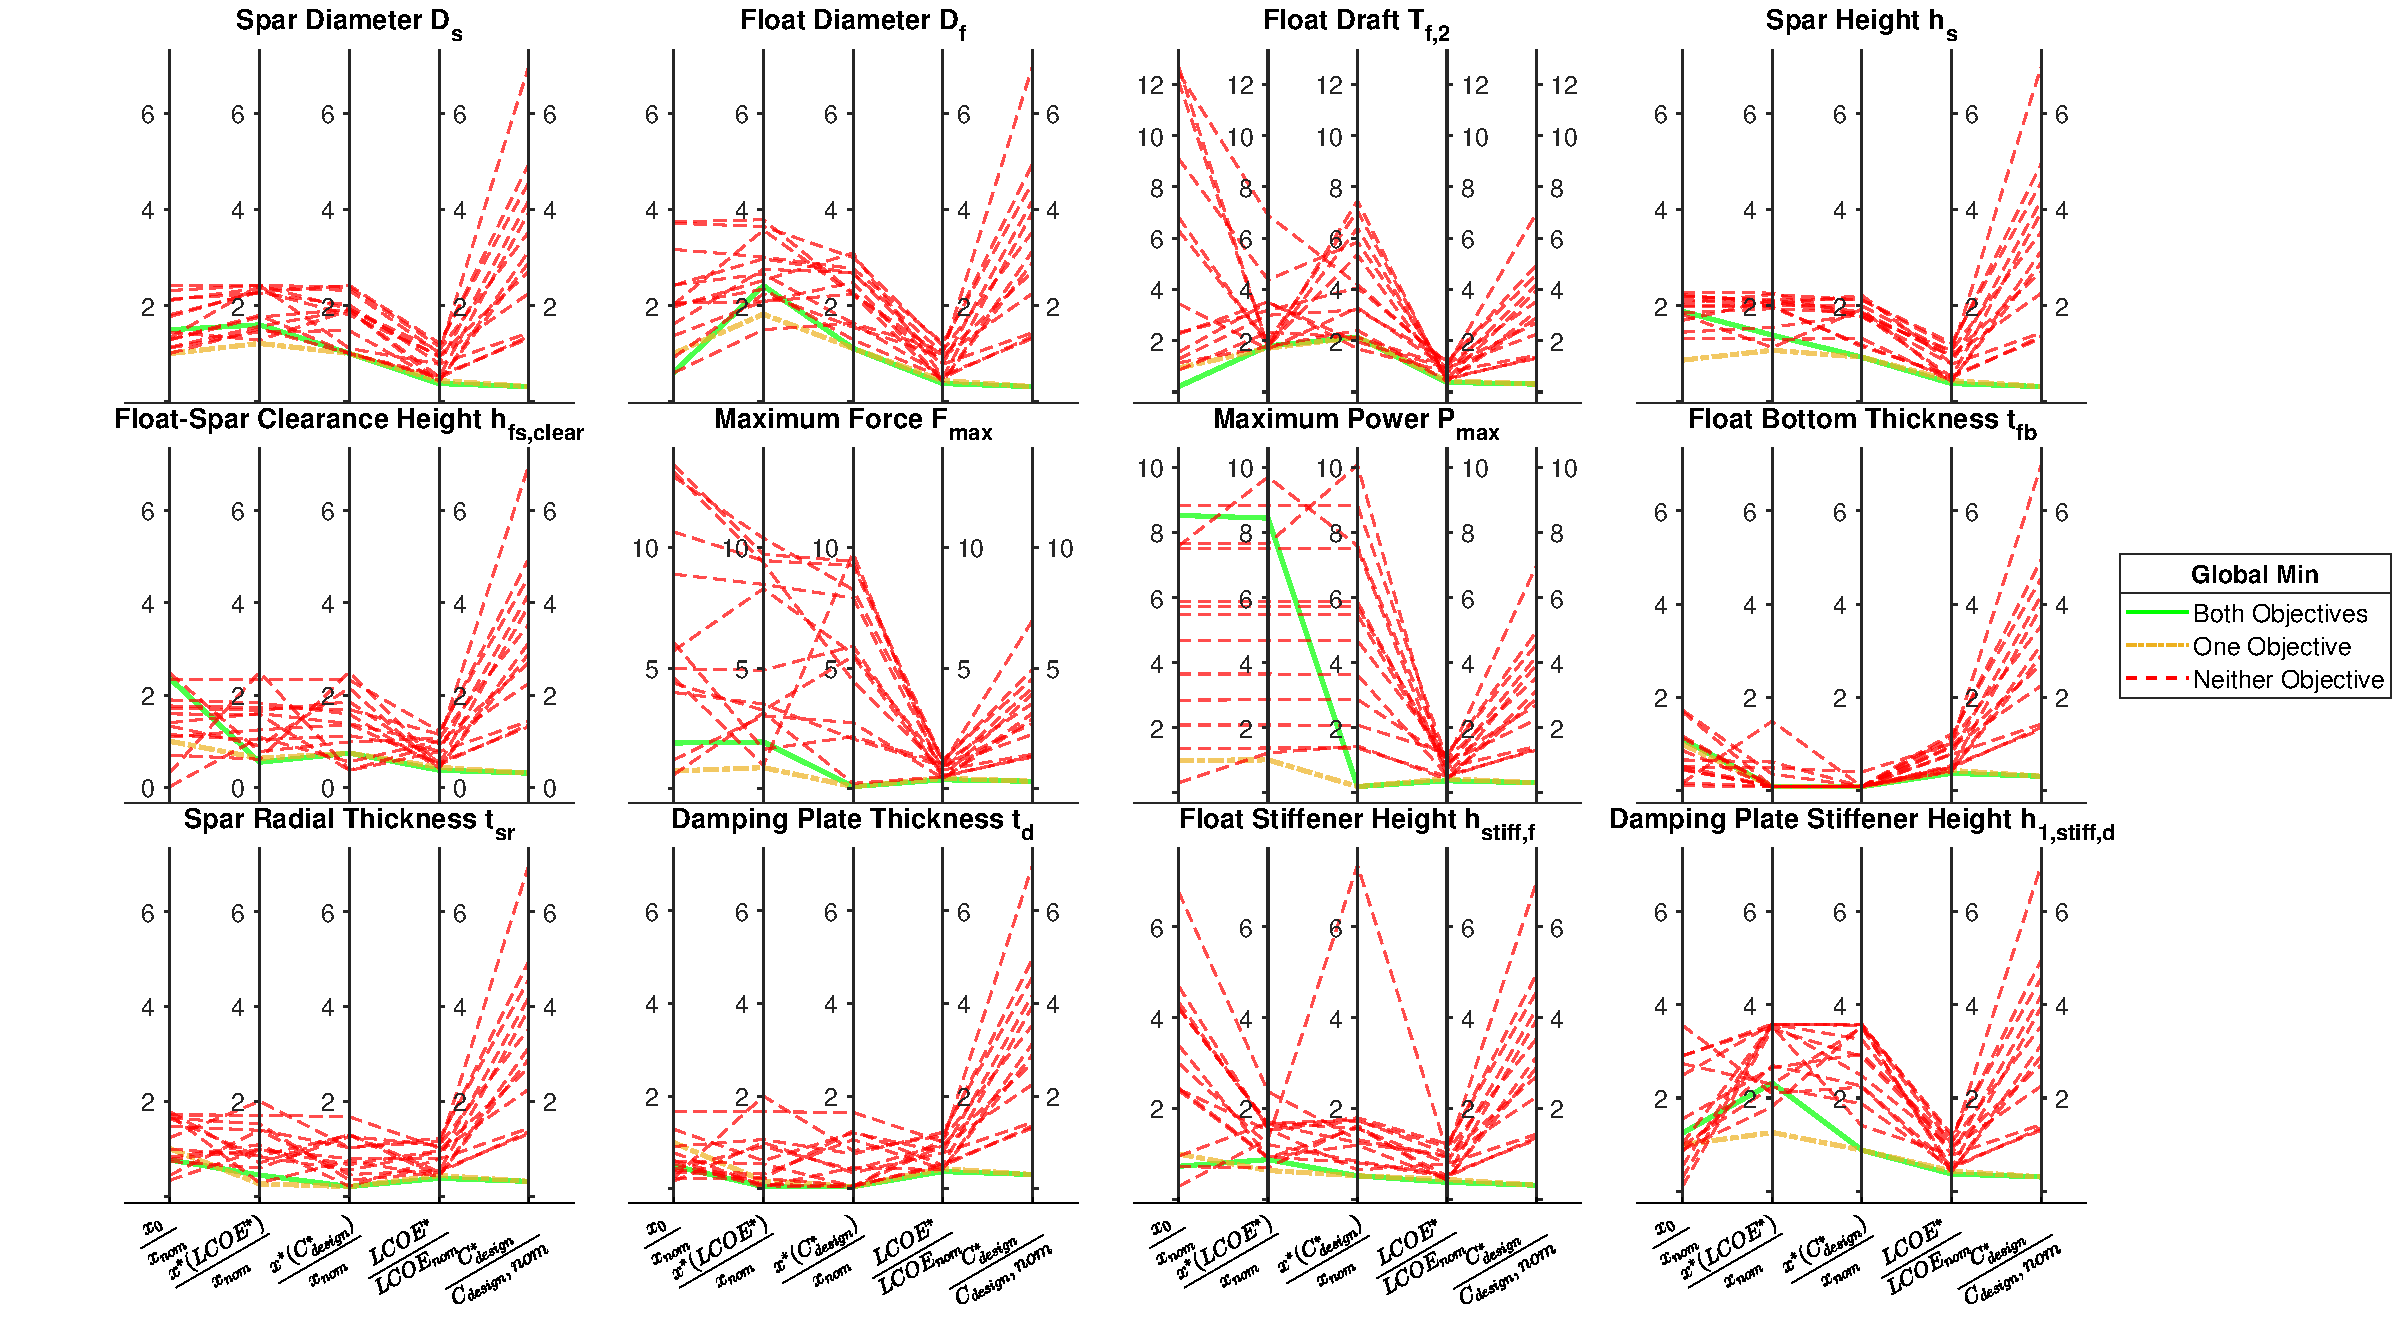
\includegraphics[width=1.2\linewidth]{figs/multistart_parallel_axis.pdf}
\caption{Parallel axis plot for effect of starting point on convergence}\label{fig:multistart-parallel-axis}
\fillandplacepagenumber
\end{figure}

\endgroup
\end{landscape}

\end{appendices}